\documentclass{article}

\usepackage[top=3cm, bottom=3cm, left=3cm, right=3cm]{geometry}

\usepackage[french]{babel}
\usepackage[utf8]{inputenc}
\usepackage[T1]{fontenc}

\usepackage[a4paper,colorlinks,linkcolor=darkgray,citecolor=red,urlcolor=blue]{hyperref}
\usepackage{pdfpages}
\usepackage{graphicx}
\usepackage{caption}
\usepackage{amsthm}
\usepackage{listings}
\usepackage{tikz}
\usepackage{algorithm}
\usepackage{amsmath}
\usepackage[noend]{algpseudocode}
\usepackage{amsfonts}
\usepackage{amssymb}

\usetikzlibrary{calc, trees, positioning, arrows, shapes,
  shapes.multipart, shadows, matrix, decorations.pathreplacing,
  decorations.pathmorphing, automata}
\definecolor{vert}{RGB}{0,153,0}

\newtheorem{ex}{Exemple}

\title{Rapport final : TriComp}

\author{}

\date{Vendredi 19 Décembre 2014}

\begin{document}

\lstset{
     literate=%
         {é}{{\'e}}1
}

\makeatletter % Pour utiliser le "at" comme une commande interne.
  \begin{titlepage}
    \begin{center}
       {\LARGE \@title} \\
       \vspace{2cm} {\large \@date}
       \vspace{3cm}
    \end{center}
       {\large {William \textsc{Aufort} \hfill Julien
           \textsc{Bensmail} \\}
    \vspace{1cm} {\hfill coordinateur \\} {Agathe \textsc{Herrou}
      \hfill Romain \textsc{Labolle} \\}
       \vspace{1cm} {chef de projet \\}
       \vspace{1.5cm} {Frédéric \textsc{Lang} \hfill Maxime
         \textsc{Lesourd} \\} {Laureline \textsc{Pinault} \hfill Léo
         \textsc{Stéfanesco} \\}}
       \vspace{2.5cm}
    \begin{abstract}
Ce document présente le rapport final de notre projet TriComp. Nous y détaillons tout le travail 
que nous avons effectué ainsi que les améliorations auxquelles nous avons pensé.
    \end{abstract}
  \end{titlepage}
\makeatother

\newpage

\tableofcontents

\newpage

\section*{Introduction}

Le tricot est un art que l'on imagine souvent réservé aux personnes
âgées.

Les magazines de tricot présentent souvent des modèles à réaliser
soi-même, combinant différents points. Il est cependant vite
fastidieux d'écrire la suite des instructions à suivre pour réaliser
une pièce. Notre but ici était donc de réaliser un logiciel permettant
d'une part de décrire des pièces de tricot de manière
\emph{user-friendly}, et, à partir de cette description, de générer
une suite d'instructions à destination du tricoteur permettant de
réaliser la pièce en question.

Cette opération de traduction d'un langage de ``haut niveau''
(l'ensemble des pièces du tricot) vers un langage de ``bas niveau''
(les instructions) rappelait fortement le principe d'un compilateur,
c'est pourquoi nous avons d'abord considéré notre projet comme un
``compilateur de tricot''. À l'instar de la compilation d'un langage
de programmation informatique, cette compilation de tricot était
susceptible de mener à des problèmes théoriques intéressants, à mesure
que l'on enrichirait le langage.

\subsection*{Notions du tricot} % ou : Quelques mots sur le tricot

% définition d'un certain nombre de mots : maille, point, ouvrage ; et description rudimentaire des techniques

Le vocabulaire du tricot peut sembler un peu obscur aux non-initiés.
Voici donc quelques définitions qui seront utiles pour la compréhension
de la suite du rapport :

\begin{itemize}
% + rang
\item[$\bullet$] une \emph{maille} est l'unité de base d'un tricot. Il s'agit de
  la boucle qui constitue l'étoffe en étant reliée à ses voisines,
  horizontalement car partageant la même portion de fil, verticalement
  car ces boucles sont imbriquées les unes dans les autres. Elle peut
  être à l'endroit ou à l'envers, selon la manière dont la boucle est
  réalisée. La figure \ref{maille} montre comment sont composées des mailles
  et les rangs.

\begin{figure}[!ht]
  \centering 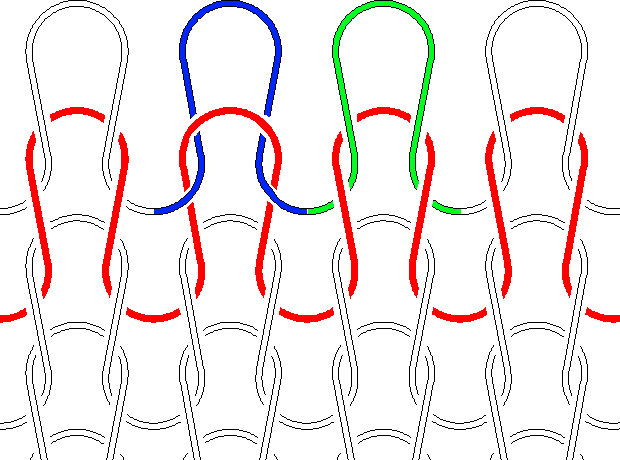
\includegraphics[scale=0.25]{../presentation/Knit-schematic2.png}
  \caption{Un schéma sur une partie de tricot, où l'on peut observer des rangs 
  (en rouge), ainsi que des mailles endroit (en vert) et envers (en bleu)}
  \label{maille}
\end{figure}

\item[$\bullet$] un \emph{point} est une manière de combiner les différentes
  opérations réalisables sur les mailles (les tricoter à l'endroit, à
  l'envers, en tricoter plusieurs ensemble, croiser plusieurs mailles
  \dots) Ceci montre que l'on peut obtenir un nombre de motifs possibles 
  extrèmement important.
\item[$\bullet$] l'\emph{ouvrage} désigne la pièce de tricot tout entière, par
  exemple l'écharpe ou le pull.
\item[$\bullet$] une \emph{diminution} est la suppression d'une maille dans le
  cours de l'ouvrage ; une technique courante consiste à tricoter
  ensemble deux mailles. Symétriquement, une \emph{augmentation} est
  une maille ajoutée dans le cours de l'ouvrage ; une technique
  courante consiste à enrouler le fil sur l'aiguille pour former une
  nouvelle maille (on parle alors de \emph{jeté}).
\end{itemize}

Le tricot est réalisé à l'aide d'aiguilles, qui servent d'une part à
maintenir les boucles libres (pour éviter qu'elles ne se défassent et
libèrent les boucles du rang précédent qu'elles retiennent), d'autre
part à former de nouvelles boucles.

\newpage

\section{Travail réalisé}

Le travail que nous prévoyions de réaliser impliquait d'une part de
définir différents langages de ``programmation'' du tricot (un langage
de haut niveau pour décrire de manière rigoureuse les ouvrages, et un
langage de bas niveau correspondant aux mailles à tricoter), d'autre
part d'écrire un compilateur réalisant la traduction d'un langage vers
l'autre, et enfin de réaliser une interface graphique permettant de
les manipuler intuitivement et de visualiser les pièces en cours de
définition.  Nous détaillons dans cette partie le travail qui a été
réalisé dans chacun de ces objectifs. Nous rappelons que tout le
travail (logiciel, documents et site web) sont disponibles et
consultables sur le dépôt Git du projet
TriComp. (\url{https://github.com/TriComp/}).

\subsection{Définition des langages}

Nous avons été amenés au cours de ce projet à définir deux langages,
l'un purement statique, puisque servant à décrire les ouvrages de
tricot, l'autre dyamique, car décrivant le processus de réalisation du
tricot. Nous les détaillons maintenant.

\subsubsection{Langage descriptif}

Une première version du langage descriptif avait été détaillée dans le
rapport mi-parcours. Quelques modifications ont été effectuées
depuis. Nous exposerons donc ici le langage final, les modifications
effectuées ainsi que leur intêret, le tout illustré par un exemple. \\

L'idée générale est de concevoir une langage capable décrire un tricot
de la façon la plus globale possible. Dans les (rares) logiciels de
tricot qui existent, le tricot est décomposé en sa plus petite entité
: la maille (cf figure \ref{logiciel}). L'avantage de cette
décomposition atomique est que l'on peut réaliser des choix de points
avec une très bonne précision.
 Son gros inconvégniant est qu'il est souvent
pénible de travailler avec cette représentation trop précise, car les tricots 
sont souvent d'assez grande taille. % TODO Une idée de la taille d'un tricot "classique"?
Notre démarche, quand à elle, propose une vision du tricot plus globale, 
et donc beaucoup plus simple.

\begin{figure}[!ht]
  \centering 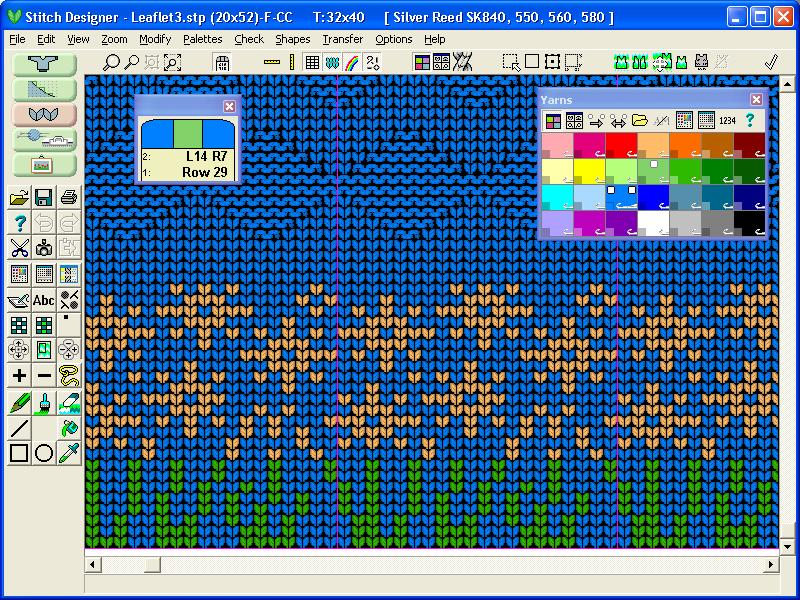
\includegraphics[scale=0.3]{../img/grid.jpg}
  \caption{Le logiciel Stitch Designer propose une vue très précise du
    tricot, mais celui-ci a donc une taille beaucoup trop importante
    (comme en témoignent les barres de défilement à droite et en bas
    de la fenêtre)}
  \label{logiciel}
\end{figure}

L'élément de base dans ce langage est le trapèze. Un trapèze définit
une zone où l'on trouve un même motif. Un trapèze est défini par sa
hauteur, le décalage de sa base supérieure, et la longueur de ses
bases (voir figure \ref{trapeze}).

\begin{figure}[!ht]
  \centering 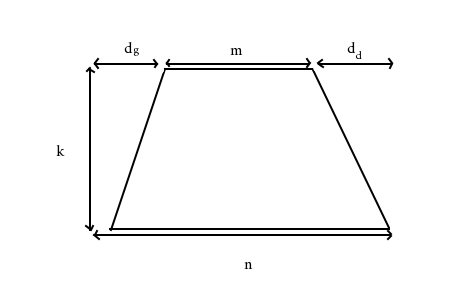
\includegraphics[scale=0.5]{../img/trapeze.jpg}
  \caption{Les paramètres d'un trapèze que l'on utilise dans la
    description}
  \label{trapeze}
\end{figure}

Un tricot est subdivisé en trapèzes qui sont reliés les uns les autres
d'une certaine manière : un trapèze connaît l'entité qui le suit
directement (dans le parcours du tricot) via un pointeur. Il se peut
que plusieurs trapèzes suivent un même trapèze : c'est dans cette
situation que l'on ajoute des aiguilles. Cette situation se modélise
dans le langage via le mot-clé "\texttt{split}".  Inversement, il se
peut que plusieurs trapèzes aient le même successeur, c'est à ce
moment là que plusieurs "morceaux" peuvent être réunis afin de libérer
une ou plusieurs aiguilles : c'est un "\texttt{link}".

Notre format de fichier nous autorise à définir différentes pièces
avec différents noms. Ces pièces permettent de décomposer une pièce,
notamment en cas de présence de \texttt{link}, qui prennent en entrée
le nom de la pièce suivante.

La figure \ref{langage} illustre et résume les possibilités du
langage, via une description d'un poncho.
\begin{figure}[!ht]
	\centering
	\begin{tikzpicture}[scale = 0.05]
		\tikzstyle{fleche}=[->,>=latex,line width=1mm]
                \fill[color=gray!20] (0,0) -- (60,0) -- (60,120) --
                (0,120) -- cycle; \fill[color=white] (30,30) --
                (45,60) -- (30,90) -- (15,60) -- cycle; \draw[thick]
                (0,0) -- (60,0) -- (60,120) -- (0,120) -- cycle;
                \draw[thick] (0,30) -- (60,30) ; \draw[thick] (0,90)
                -- (60,90) ; \draw[thick] (0,60) -- (15,60) ;
                \draw[thick] (45,60) -- (60,60) ; \draw[thick] (30,30)
                -- (45,60) -- (30,90) -- (15,60) -- cycle;
                \draw[fleche, color=red] (30,20) -- (15,40);
                \draw[fleche, color=red] (30,20) -- (45,40);
                \draw[color=red] (30,15) node{split}; \draw[fleche,
                  color=blue] (8,50) -- (8,70); \draw[fleche,
                  color=blue] (52,50) -- (52,70); \draw[color=blue]
                (30,60) node{next}; \draw[fleche,color=vert] (15,80)
                -- (30,100); \draw[fleche,color=vert] (45,80) --
                (30,100); \draw[color=vert] (30,105) node {link};
                \draw (30,-10) node{start}; \draw[fleche] (30,-5) --
                (30,10); \draw (30,130) node{stop}; \draw[fleche]
                (30,110) -- (30,125); \draw[-*,ultra thick] (75,30) --
                (45,15); \draw (90,35) node{\texttt{trapeze(...)}};
	\end{tikzpicture}
	\caption{Les possibilités du langage illustré sur un tricot
          (en l'occurence un poncho). Une attention toute particulière
          est portée aux jonctions entre les différents trapèzes.}
	\label{langage}
\end{figure}

Comme nous le disions précédemment, quelques modifications ont été
apportées au niveau de ce langage depuis le rapport de
mi-parcours. Deux choses importantes ont été modifiées :
\begin{itemize}
	\item La largeur inférieure des trapèzes est cette fois-ci
          déduite de la largeur de la pièce précédente, et ne figure
          donc plus dans les paramètres du trapèze. Cette modification
          permet d'éviter des redondances sans se compliquer la tâche,
          notamment dans la partie de l'interface graphique.
	\item Les \texttt{split} peuvent générer plus de deux pièces
          différentes. Par conséquent, les \texttt{links} ont
          également été modifiés : ils se lient avec leur sucesseur
          via le nom du sucesseur, suivi de la position sur ce
          sucesseur (alors qu'avant, un simple positionnement
          gauche/droite suffisait). Nous avons effectué cette
          modification car certains tricots (par exemple la salopette)
          ne pouvait être écrit de façon "simple" avec le précédent
          langage. Ceci est du au fait que précédemment, le
          positionnement des pièces après un split était déterministe
          (une pièce à gauche, une pièce à droite) et donc
          restrictif. Cette partie a apporté beaucoup plus de
          modifications dans le code que la modification précédente.
\end{itemize}

Au final nous obtenons un langage permettant de représenter une quantité importante 
de tricots d'un point de vue assez original par rapport à ce qui est fait dans les 
autres logiciels de tricot. Les tricots qui suivent notre langage portent l'extension 
\texttt{.tricot}.

\subsubsection{Langage de bas niveau}

Le "langage de bas niveau" correspond aux instructions que doit suivre l'utilisateur 
pour pouvoir réaliser son tricot. Ces instructions sont produites par le compilateur, 
dont on détaillera le fonctionnement dans la prochaine partie. Ici nous présentons le 
format (ou langage) utilisé pour présenter ces instructions, en effectuant un parallèle 
avec ce que l'on peut trouver dans un manuel de tricot.

Ce langage doit reflèter exactement les mêmes informations que celles que l'on pourrait 
trouver dans un manuel de tricot : les points à tricoter. Dans les manuels, la périodicité 
des motifs est exploitée afin de ne pas créer une instructions pour chaque maille. Cette 
périodicité se traduit à la fois sur un rang (hoirzontalement, voir la figure \ref{instruction1}) 
et sur un ensemble de rangs (verticalement, voir la figure \ref{instruction2}).  

\begin{figure}[!ht]
	\centering
	\fbox{\begin{minipage}{0.9\textwidth}
	\begin{lstlisting}^^J
Ligne 1 : 140 fois 1 maille endroit, 1 maille envers^^J
	\end{lstlisting}
	\end{minipage}}
	\caption{Ici, on repète une succession de points plusieurs fois sur un même rang.}
	\label{instruction1}
\end{figure}

\begin{figure}[!ht]
	\centering
	\fbox{\begin{minipage}{0.9\textwidth}
	\begin{lstlisting}^^J
Répetez 245 fois le motif suivant :^^J
Ligne 1 : 140 fois 1 maille endroit, 1 maille envers^^J
Ligne 2 : 140 fois 1 maille envers, 1 maille endroit^^J
	\end{lstlisting}
	\end{minipage}}
	\caption{Ici, on repète une succession de rangs plusieurs fois (verticalement).}
	\label{instruction2}
\end{figure}

Les deux figures précédentes illustrent des instructions que nous obtenons avec notre logiciel. 
Dans un manuel de tricot, elles sont volontairement moins verbeuses, à cause du nombre important 
de motifs différents à décrire qu'ils contiennent.

Mais tout tricot ne peut être construit uniquement à partir d'instructions de ce type. En effet, nous 
avons vu qu'avec les \texttt{split} et les \texttt{link} il est possible de devoir ajouter (ou enlever) 
une ou plusieurs aiguilles, et cette information doit figurer parmi les instructions renvoyées.

Enfin, la dernière information importante concerne le début du tricot. En effet, pour commencer un tricot, 
le tricoteur doit \emph{monter des mailles}. Ces premières mailles sont particulières, car elles ne 
reposent pas sur des mailles précédemment tricotées. Nous indiquons donc au début du tricot le nombre de 
mailles à monter. Cette étape ne figure pas dans les manuels de tricot, car ceux-ci traitent souvent de 
motifs, et non de pièces.

Ainsi, les instructions que renvoit notre logiciel sont à la fois précises comme celles d'un manuel, mais 
également claires et facile à suivre. 

\subsection{Compilateur}

\subsubsection{Parcours du tricot}

Le parcours du tricot utilise l'algorithme 1, qui est un algorithme de
dataflow à work list, très courant en compilation. Ici le workset est
implémenté à l'aide d'une pile, ce qui nous permet de parcourir
complètement une branche de tricot avant de s'occuper d'une
autre. Ainsi on ne demande pas au tricoteur de faire un va-et-vient
entre plusieurs aiguilles si ce n'est pas nécessaire.

\begin{algorithm}\label{algo}
\caption{\textsc{Algorithme de parcours du tricot}}
\begin{algorithmic}[1]
\State WorkSet $\leftarrow$ racines du graphe.
\State Done $\leftarrow$ ($\lambda n \to \varnothing$) // Un dictionnaire
\While{$WorkList \neq \varnothing$}
  \State x $\leftarrow$ Pop\,(WorkList)
  \State Imprimer les instructions pour x
  \For{y $\in$ Successors(x)}
    \State Done(y) $\leftarrow$ Done(y) $\cup$ \{ x \}
    \If{Done(y) $=$ Predecessors(y)} // On a parcouru toutes les dépendances de x
      \State WorkSet $\leftarrow$ WorkSet $\cup$ \{ y \}
    \EndIf
  \EndFor


%  \If{$i = \{r \leftarrow \phi (x_1, \dots, x_k)\}$}
%    \State newval $\leftarrow \SBabrs{x_1}{lv} \sqcup \cdots \sqcup \SBabrs{x_k}{lv}$
%  \ElsIf {$i = \{r \leftarrow x ~ op ~ y\}$}
%    \State newval $\leftarrow \SBabrs{x ~ op ~ y}{lv}$
%  \EndIf
%  \If{$($newval $\sqcup$ $\SBabrs{r}{lv}) \neq \SBabrs{r}{lv}$}
%    \State lv\,[$r$] $\leftarrow$ newval $\sqcup$ $\SBabrs{r}{lv}$
%    \State WorkList $\leftarrow$ WorkList $\cup$ DefUse($r$)
%  \EndIf
\EndWhile

%\State $WorkList \leftarrow map ~(\lambda (v : L) \to (v = \bot) ? \, \top : v) ~ WorkList$
\end{algorithmic}
\end{algorithm}

\subsubsection{Etapes de vérifications}

\subsection{Interface graphique}

Nous exposons dans cette partie le travail qui a été fourni concernant
l'élaboration de l'interface graphique, notamment les caractéristiques
de l'interface, les fonctionnalités ainsi que des détails
d'implémentation.

\subsubsection{Caractéristiques et fonctionnalités}

Avant toute chose, il nous fallait cibler les caractéstiques que
devait avoir l'interface. Destinée à être utilisée par des tricoteurs,
celle-ci devait être facile d'utilisation. L'utilisateur dispose des
outils indispensables à toute interface (ouverture, sauvegarde de
fichiers, zoom...) mais également d'outils propres au tricot et aux
objectifs de TriComp : un bouton pour générer les instructions, ainsi
que quelques outils d'édition de tricot (choix des points sur les
trapèzes).

Le choix du motif à mettre sur chaque trapèze peut être fait parmi une
dizaine de points disponibles via des boutons. Une suggestion future
pourrait être de faire définir à l'utilisateur ses propres points.

L'interface est divisée en trois parties : une partie contenant les
outils d'édition de tricot, une fenêtre où est affiché le tricot, et
une zone où se trouve la liste des instructions générées par le
compilateur.

% TODO : inclure des images 

\subsubsection{Détails d'implémentation}

L'interface a été créée à l'aide de la bibliothèque Qt. Une grande
partie du projet a été intégrée au sein de la partie Qt, pour des
questions de simplificité au niveau de l'intégration. Seule la partie
compilation (écrite en OCaml) est dissociée de la partie Qt, et est
appelée dans l'interface via des appels systèmes.

Détailler l'ensemble des structures offertes par Qt utilisées dans le projet
serait ici long et inutile, le lecteur pourra se référer au code
disponible sur la page Github\footnote{Rappel :
  \url{https://github.com/TriComp/}}. On mentionnera juste que pour
l'affichage, on ne travaille pas directement sur le tricot en temps
qu'objet, mais sur une représentation du tricot formée
d'\texttt{items} (qui forme, en quelque sorte, une couche
supérieure). Même si les deux représentations sont isomorphes
(grossièrement un \texttt{item} pour un trapèze du tricot), cela
permet d'éditer autant qu'on le veut sans modifier l'objet de base
(sauf lors d'une sauvegarde).

\subsection{Communication}

Nous détaillons dans cette partie la partie communication du projet,
qui englobe la communication interne et externe (via le site web).

\subsubsection{Site Web}

Un site web a été déployé à l'adresse \url{http://tricomp.github.io}, il est hébergé
sur Github (utilisé comme serveur Git du projet). Le site est basé sur Jekyll, un 
CMS en Ruby spécialisé dans les blogs et qui a la particularité de ne pas utiliser 
de base de données, avec l'avantage que Github gère Jekyll automatiquement. Le site 
est notamment une vitrine pour le projet : il en contient une présentation rapide, 
avec des liens vers le code source sur Github, ainsi que différents articles autour du projet.
La page dispose également d'une page pour aiguiller rapidement l'internaute anglophone

% TODO un onglet téléchargement ?

\subsubsection{Communication au sein du projet}

La communication au sein du projet s'est principalement effectuée par le biais de notre liste
de diffusion (tricomp [at] listes.ens-lyon.fr). L'échange des idées au début du projet s'est 
fait par l'intermédiaire d'un pad hébergé par l'association AliENS (\url{http://pad.aliens-lyon.fr/p/tricomp}). 
Nous nous réunissions également toutes les semaines avec notre encadrant afin de faire le point 
sur l'avancement du projet, de discuter de choix, tels que la syntaxe du langage descriptif, 
la modélisation à adopter pour les points, les fonctionnalités du logiciel final\dots

\section{Améliorations possibles}

Le manque de temps et de moyens humains nous a empêché de mettre en
place la totalité des fonctionnalités que nous avions prévues. Nous détaillons
ici quelques améliorations auxquelles nous avons songées, sachant qu'elles veront
peut-être le jour (certaines personnes de l'équipe étant intéressées par la 
poursuite du projet).

\subsection{Langage descriptif}

En ayant plus de temps à notre disposition, nous pourrions intégrer au
langage d'une part les diminutions et augmentations, d'autre part les
tresses. De même, une fois le tricot terminé, il faut en général le
finaliser en cousant certaines parties. Cette dernière étape de
couture avait été évoquée, mais n'a pas été traitée. Toutefois, la
difficulté de cette étape (en matière de tricot) n'est pas très
importante pour un tricoteur.

\subsection{Compilateur}

Le compilateur actuel ne gère que les rectangles. La gestion des trapèzes 
(l'idée centrale du langage) serait un des premiers points sur lequel nous
pourrions nous pencher de nouveau. A travers cette qestion se pose notamment
les problèmes dela gestion des augmentations et des diminutions, notamment pour
des motifs complexes.

\subsection{Interface graphique et édition}

Du côté de l'interface, une grande partie du travail que nous n'avons
pas eu le temps d'aborder portait sur l'édition des tricots. Nous
avions pensé notamment à la définition de points par l'utilisateur, à
pouvoir changer la taille des pièces, ou encore améliorer le rendu des
points. L'insertion de points particuliers sur des zones (par exemple,
des tresses) aurait pu être un outil intéressant à implémenter.

\section{Résultats théoriques}

\subsection{Algorithmes de répartition des diminutions}

Dans l'optique d'intégrer des trapèzes non rectangulaires au langages, nous nous sommes penchés sur la manière de répartir des 
diminutions et augmentations au cours des rangs afin que les côtés apparaissent rectilignes.

Nous nous sommes donc penchés du côté des algorithmes d'image, 

\subsection{Allocation d'aiguilles}

Lors de la génération des instructions, on souhaiterait déterminer le nombre d'aiguilles nécessaires à la réalisation du tricot, 
et si possible le minimiser. Ce problème ressemble fort à celui de l'allocation de registres en compilation, et on peut montrer 
qu'il lui est en fait équivalent.

En effet, faisons l'analogie suivante : on fait correspondre les aiguilles supplémentaires (par rapport aux 2 aiguilles de base) 
aux temporaires dans lesquels stocker les variables, et les variables aux zones où le tricot est séparé en deux, introduites par 
les \texttt{split} (en gardant en tête qu'on peut évidemment effectuer un \texttt{split} sur une branche déjà issue d'un \texttt{split}).

\section*{Conclusion}

Au terme des quatre mois qui nous étaient donnés pour mettre en place le logiciel, nous avons créé un langage robuste ainsi un 
logiciel fonctionnel sur les différentes parties (compilateur, interface), ce dernier étant cependant incomplet par rapport aux 
objectifs que nous nous étions fixés en début de projet. La partie implémentée répond au besoin primaire que nous avions ciblé : 
la génération d'instructions relatives à un tricot via une interface graphique.

\end{document}
